%---------------------------------------------------------------------------
%	Packages
%---------------------------------------------------------------------------
\documentclass[twocolumn]{article}
\usepackage[utf8]{inputenc}
\usepackage[english]{babel}
\usepackage{amsmath}
\usepackage{authblk}
\usepackage{background}
\usepackage{fancyhdr}
\usepackage[left = 1.5cm, right = 1.5cm, top = 2cm, bottom = 2cm]{geometry}
\usepackage{graphicx}
\usepackage[hidelinks]{hyperref}
\usepackage{indentfirst}
%---------------------------------------------------------------------------
%	Header / Footer / Background
%---------------------------------------------------------------------------
\pagestyle{fancy}
\fancyhead[L]{Taylor Larrechea}
\fancyfoot[L]{PHYS 342}
\fancyhead[C]{Three Body Problem}
\fancyhead[R]{Colorado Mesa University}
\fancyfoot[R]{Final Project}
\backgroundsetup{
    scale = 1,
    angle = 0,
    opacity = 0.1,
    contents = {
    
\includegraphics[scale = 0.5, keepaspectratio]{Figures/CMU Seal.png}
    }
}
%---------------------------------------------------------------------------
%	Document Info
%---------------------------------------------------------------------------
\title{\textbf{Dynamics of a Triple Star System}}
\author{Taylor Larrechea \\ Colorado Mesa University \\
    Department of Physical and Environmental Sciences \\
    1100 North Avenue \\
    Grand Junction, CO 81501-3122
}
\date{December 11, 2018}
%---------------------------------------------------------------------------
%	Document
%---------------------------------------------------------------------------
\begin{document}
%---------------------------------------------------------------------------
%	Abstract
%---------------------------------------------------------------------------
\twocolumn[
    \begin{@twocolumnfalse}
        \maketitle
        \begin{abstract}
            This article reports the examinations of a three body star orbit. These orbits are impossible to solve analytically and require numerical methods for plotting the orbits of these stars. Precisely, python and a Forward Euler Difference Scheme (Or F.E.D.S for short) was used to solve for these stars' equations of motion. After these solutions were found, it was observed that these three body orbits are primarily unstable with only specific initial conditions yielding stable orbits of the three stars.
        \end{abstract}
    \end{@twocolumnfalse}
]
%---------------------------------------------------------------------------
%	Introduction
%---------------------------------------------------------------------------
\section{Introduction}
\indent As stated in the abstract, the purpose of this report is to report the findings of the solutions for a three body orbit. To do this, the situation of a ball falling from some designated height must be looked at first. One dimensional gravitational attraction is the simplest form of gravity that can be examined. This situation lays the groundwork for the inevitable scenarios that follow in complexity. After the one dimensional motion of a ball falling to the ground is covered, the two body system will be covered. By two body it is implied that there are only two bodies in space where the only force acting on these bodies are the gravitational attraction due to the other body. Once the two body system is solved, the three body will be solved and plotted for as well.

The studying of the three body problem dates all the way back to 1499 when Amerigo Vespucci and Galileo Galilei first attempted to solve for these equations of motion \cite{BodyWiki}. Unfortunately, for both Amerigo and Galileo were naive and did not know that their efforts were essentially being wasted. Amerigo and Galileo were wasting their time because the force equations that are derived for these bodies in space have too many variables changing to be able to solve for analytically. Since the position of these orbits are time dependent, it should be expected that the velocity and acceleration are time dependent as well. But along with these values being time dependent, these values are also position dependent and thus makes it impossible to solve for analytically. And queue the twentieth and twenty-first century scientists!
%---------------------------------------------------------------------------
%	Force Equations
%---------------------------------------------------------------------------
\section{Force Equations}
Before the equations of motion can be solved, we begin with Newton's second law. Isaac Newton's second law states, 'A body acted upon by a force moves in such a manner that the time rate of change of momentum equals the force.' \cite{Marion}. In mathematical terms Newton's second law is
%---------------------------------------------------------------------------
%	Equation 1 - Newtons 2nd Law
%---------------------------------------------------------------------------
\begin{equation}\label{Eqn. Newtons 2nd Law}
\Vec{F}=\frac{d\Vec{P}}{dt}=m\frac{d\Vec{V}}{dt}.
\end{equation}
Although Newton's second law involves the change of momentum of an object, we are only concerned about when the velocity is changing in the momentum. In essence, one of the equations for force that we will be using is $\Vec{F}=m\Vec{a}$, which is the last part that can be seen in equation (\ref{Eqn. Newtons 2nd Law}). It should be noted that the letters with arrows on top i.e $\Vec{F}$, $\Vec{P}$, $\Vec{V}$ all indicate vector quantities. Because of the vector nature of force, an equivalent way to write equation (\ref{Eqn. Newtons 2nd Law}) is
%---------------------------------------------------------------------------
%	Equation 2 - Newtons 2nd Law Vector
%---------------------------------------------------------------------------
\begin{equation}\label{Eqn. Newtons 2nd Law Vector}
\Vec{F}=m(\frac{d\Vec{V}}{dx}\Vec{i} + \frac{d\Vec{V}}{dy}\Vec{j} + \frac{d\Vec{V}}{dz}\Vec{k})
\end{equation}
Knowing that force is a vector sum we can use the principle of superposition and an equivalent way to write equation (\ref{Eqn. Newtons 2nd Law}) is
%---------------------------------------------------------------------------
%	Equation 3 - Newtons 2nd Law Equivalent
%---------------------------------------------------------------------------
\begin{equation}\label{Eqn. Newtons 2nd Law Equivalent}
\Vec{F}=\sum_{i=1}^{3} \frac{d\Vec{P}_i}{dt}=m\sum_{i=1}^{3} \frac{d\Vec{V}_i}{dt}
\end{equation}
where (\ref{Eqn. Newtons 2nd Law Equivalent}) gives a final mathematical definition of Newton's second law. Equation (\ref{Eqn. Newtons 2nd Law Equivalent}) has the summation go from 1 to 3 due to there only being 3 spatial dimensions in our universe. Space is of most interest in this project since star orbits are being calculated. It is also important to define what the force for gravitational attraction between two bodies is. The equation for force due to gravitational attraction is \cite{Marion}
%---------------------------------------------------------------------------
%	Equation 4 - Force Attraction
%---------------------------------------------------------------------------
\begin{equation}\label{Eqn. Force Attraction}
\Vec{F}=-\frac{GmM}{r^2} (\Vec{n})
\end{equation}
where \textit{G} is the gravitational constant, \textit{M} is the mass of the larger body, \textit{m} is the mass of the smaller body, \textit{r} is the separation between the two bodies of mass, and $\Vec{n}$ is a unit vector. Because force is a vector quantity, each individual component of the force will have to be analyzed. The distance between two points in space \textit{r} is $\textit{r}=\sqrt{x^2+y^2+z^2}$ which is abbreviated in equation (\ref{Eqn. Force Attraction}) with just an \textit{r}. The unit vector $\Vec{n}$ is  $\Vec{n}=\frac{x\Vec{i}+y\Vec{j}+z\Vec{k}}{\sqrt{x^2+y^2+z^2}}$ when combined with the distance between two points in space gives
%---------------------------------------------------------------------------
%	Equation 5 - Force Attraction Vector
%---------------------------------------------------------------------------
\begin{equation}\label{Eqn. Force Attraction Vector}
\Vec{F}=-\frac{GmM}{r^3}(x\Vec{i}+y\Vec{j}+z\Vec{k}).
\end{equation}
Equation (\ref{Eqn. Force Attraction Vector}) is used to solve for the equations of motion. Equation (\ref{Eqn. Newtons 2nd Law Vector}) and (\ref{Eqn. Newtons 2nd Law Equivalent}) can be combined to yield three separate individual force equations. One for each direction ($\Vec{i}$, $\Vec{j}$, $\Vec{k}$). For the x-direction the force equation becomes
%---------------------------------------------------------------------------
%	Equation 6 - 1D Force Equation X
%---------------------------------------------------------------------------
\begin{equation}\label{1D Force Equation X}
m(\frac{d\Vec{V}}{dx})(\Vec{i})=-(\frac{GmM}{r^3})x(\Vec{i}).
\end{equation}
The analog can be carried out to find the y and z-direction force equations. The y-direction is thus
%---------------------------------------------------------------------------
%	Equation 7 - 1D Force Equation Y
%---------------------------------------------------------------------------
\begin{equation}\label{1D Force Equation Y}
m(\frac{d\Vec{V}}{dy})(\Vec{j})=-(\frac{GmM}{r^3})y(\Vec{j})
\end{equation}
and the z-direction is finally
%---------------------------------------------------------------------------
%	Equation 8 - 1D Force Equation Z
%---------------------------------------------------------------------------
\begin{equation}\label{1D Force Equation Z}
m(\frac{d\Vec{V}}{dz})(\Vec{k})=-(\frac{GmM}{r^3})z(\Vec{k}).
\end{equation}
Equations (\ref{1D Force Equation X}), (\ref{1D Force Equation Y}), and (\ref{1D Force Equation Z}) will serve as the basis for finding the equations of motion of these stars in orbit.
%---------------------------------------------------------------------------
%	One-Dimensional Motion
%---------------------------------------------------------------------------
\section{One-Dimensional Motion}
Before the motion of three bodies can be solved, the simplest scenario must first be examined and extended to the initial problem. One simple example of a force attraction between two bodies of mass is a ball falling towards the surface of the Earth. Without accounting for drag, the time that it takes for an object to fall back to the Earth's surface with no initial velocity is given by 
%---------------------------------------------------------------------------
%	Equation 9 - 1D Time Equation
%---------------------------------------------------------------------------
\begin{equation}\label{1D Time Equation}
t=\sqrt{\frac{2h}{g}},
\end{equation}
where \textit{h} is the initial height near the surface of the Earth and \textit{g} is the acceleration due to gravity. A plot of \textit{h} versus \textit{t} for this ball was calculated numerically with the use of python. In general
%---------------------------------------------------------------------------
%	Equation 10 - Force Equation Y
%---------------------------------------------------------------------------
\begin{equation}\label{Force Equation Y}
m_{b}\frac{dV}{dt}=-\frac{GM_{E}m_{b}}{(R_{E}+y)^2},
\end{equation}
was used to solve for the equation of motion of the ball being dropped from a specific height. The $M_{E}$ and $R_{E}$ values are the mass and radius of the Earth respectively. Where as the $m_b$ variable is the mass of the ball that is being dropped. The variable \textit{y} in Equation (\ref{Force Equation Y}) is the initial height that the object (in this case, a ball) is being dropped from. Solving Equation (\ref{Force Equation Y}) with the initial conditions of $y_0=100$ $m$ and $V_{y0}=0$ $\frac{m}{s}$ yields the following plot seen in Figure 1 below.
%---------------------------------------------------------------------------
%	Figure 1 - 1D Position Plot
%---------------------------------------------------------------------------
\begin{figure}[ht]
    \centering
    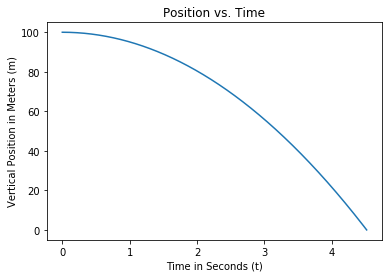
\includegraphics[width=8cm, height=5cm]{Figures/1D Position Plot.png}
    \caption{\small{Position vs. Time of Object Falling.}}
    \label{Fig. 1D Position Plot}
\end{figure}
\par \noindent
Figure \ref{Fig. 1D Position Plot} coincides with what should be observed with a ball falling towards Earth. The rate of change in Figure 1 increases with respect to time telling us that the velocity of this object is increasing as it falls towards the Earth. The acceleration is precisely \textit{g} as this ball falls, which is what should be observed.
%---------------------------------------------------------------------------
%	Force Attraction Between Two Bodies of Mass
%---------------------------------------------------------------------------
\section{Force Attraction Between Two Bodies of Mass}
One-dimensional gravitational force attraction has been examined, the next topic of discussion is two bodies of mass being attracted to one another. The scenario for this example involves two massive bodies in space being attracted towards one another from a certain distance apart.
%---------------------------------------------------------------------------
%	Figure 2 - 2-Body Cartoon
%---------------------------------------------------------------------------
\begin{figure}[ht]
    \centering
    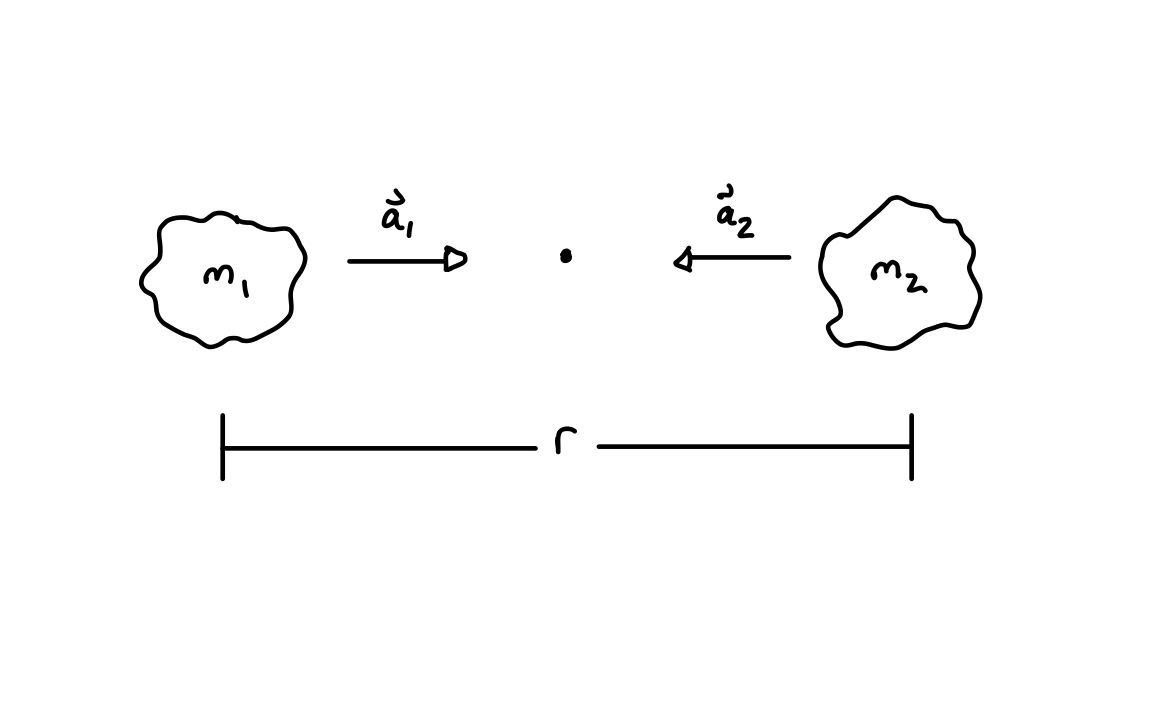
\includegraphics[width=8cm, height=5cm]{Figures/2-Body Cartoon.png}
    \caption{\small{Two Bodies In Space.}}
    \label{Fig. 2-Body Cartoon}
\end{figure}
\par \noindent
Figure \ref{Fig. 2-Body Cartoon} shows a sketch of what we are considering next. Newton's second law holds and in space the force between the two is gravitational. Using Newton's second law and the force due to gravity, the equations of motion for both object 1 and 2 can be solved. The acceleration for object 1 is thus
%---------------------------------------------------------------------------
%	Equation 11 - Object 1 Acceleration
%---------------------------------------------------------------------------
\begin{equation}\label{Eqn. Object 1 Acceleration}
a_{1}=-\frac{Gm_{2}}{r^2},
\end{equation}
where the acceleration for object 2 can be written as
%---------------------------------------------------------------------------
%	Equation 12 - Object 2 Acceleration
%---------------------------------------------------------------------------
\begin{equation}\label{Eqn. Object 2 Acceleration}
a_{2}=-\frac{Gm_{1}}{r^2}.
\end{equation}
The motion of these objects are purely in one direction (It can be interpreted as the x-direction) so the unit vector is not necessary in Equations (\ref{Eqn. Object 1 Acceleration}) and (\ref{Eqn. Object 2 Acceleration}). It should be noted that the only forces presumably acting on these bodies of mass in space is the gravitational attraction due to the other body of mass.

In the example of motion stated above in Figure 2, there are two bodies in space that are separated by an arbitrary distance apart from one another. There is a common point in which these two bodies of mass will collide into one another and this motion is the next item to be solved for. For the purpose of simplicity, the masses $M_1$ and $M_2$ were set to 50 kilograms and 100 kilograms respectively. The initial separation distance between the two was 200 meters which corresponds to the \textit{r} value found in equation (\ref{Eqn. Force Attraction Vector}). The original position of $M_1$ was at $X_{1i}=-100$m and $M_2$ was at $X_{2i}=100$m. Taking these parameters for both $M_1$ and $M_2$, the original position of these two in space looks something like this.
%---------------------------------------------------------------------------
%	Figure 3 - 2-Body Fig. 1
%---------------------------------------------------------------------------
\begin{figure}[ht]
    \centering
    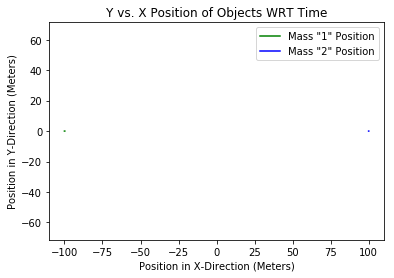
\includegraphics[width=8cm, height=5cm]{Figures/2-Body (1).png}
    \caption{\small{Initial Position of Two Bodies in Space.}}
    \label{Fig. 2-Body Fig. 1}
\end{figure}
\par \noindent
It can be seen very faintly in Figure \ref{Fig. 2-Body Fig. 1} the position of both mass $M_1$ and $M_2$. It should be noted that after a time interval the two would start attracting to one another until the point of collision. Figure 4 shows the path of this motion.
\newpage
%---------------------------------------------------------------------------
%	Figure 4 - 2-Body Fig. 2
%---------------------------------------------------------------------------
\begin{figure}[ht]
    \centering
    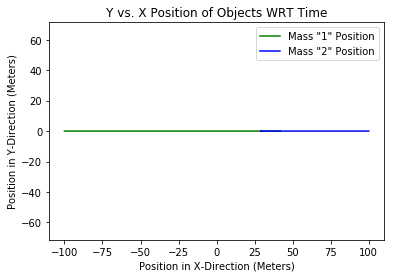
\includegraphics[width=8cm, height=5cm]{Figures/2-Body (2).png}
    \caption{\small{Two Bodies Being Attracted to One Another.}}
    \label{Fig. 2-Body Fig. 2}
\end{figure}
\par \noindent
Figure \ref{Fig. 2-Body Fig. 2} shows the distance covered in the X-direction of both of these masses. It should be noted that the green line, $M_1$, traverses a further distance in the same amount of time as the blue line $M_2$. This physically makes sense since the acceleration that is due to $M_1$ is contingent upon the separation distance and $M_2$ in the system. Therefore it would make sense that $M_1$ would cover more ground in the same time due to its acceleration being greater than $M_2$. Conversely the reason why $M_2$ traverses less than compared to $M_1$ is because its acceleration is less than that of $M_1$'s due to $M_1$ having a smaller mass than $M_2$.
%---------------------------------------------------------------------------
%	Planetary And Celestial Body Motion
%---------------------------------------------------------------------------
\section{Planetary and Celestial Body Motion}
A natural extension of gravitational attraction is orbital motion. Since the main task is the plot the orbits of three stars in space, understanding orbital motion is crucial. We first review Kepler's laws \cite{Marion}.
\begin{center}
\textbf{I}. \small{\textit{Planets move in elliptical orbits about the Sun with the Sun at one focus.}} \newline
\textbf{II}. \small{\textit{The area per unit time swept out by a radius vector from the Sun to a planet is constant.}} \newline
\textbf{III}. \small{\textit{The square of a planet's period is proportional to the cube of the major axis of the planet's orbit.}} \newline
\end{center}
The most important of these three laws to us is the first law \textbf{I}. This law states that all planetary motion about one focus should be in the shape of an ellipse. A perfect orbit in theory would be a perfect circle, this is not the case most of the time in space. For two body orbits the shape of the orbit should also be ellipses. The previous force equations that were used to solve for the equations of motion for two bodies in space can be used to solve for orbital motion. Taking a look at the inner planets, their orbits tend to be more circular than the planets that are farther from the sun. Take for instance the Earth's orbit plotted below.
\newpage
%---------------------------------------------------------------------------
%	Figure 5 - Earth Orbit
%---------------------------------------------------------------------------
\begin{figure}[ht]
    \centering
    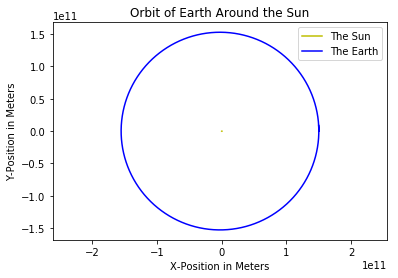
\includegraphics[width=8cm, height=5cm]{Figures/Earth Orbit.png}
    \caption{\small{One Orbital Period of Earth.}}
    \label{Fig. Earth Orbit}
\end{figure}
\par \noindent
It can be observed that the orbit in Figure \ref{Fig. Earth Orbit} is circular. This shape of orbit is not that common for celestial bodies that are farther from the sun. In fact, this shape of orbit is usually very similar for any scenario in which the orbit is very large. As the orbit is traced out over time, Earth doesn't travel much farther away from the Sun while it doesn't start to get closer to the sun as well. Compared to another planets (or dwarf planets) orbit, say Pluto, Earth is circular in its orbit.
%---------------------------------------------------------------------------
%	Figure 6 - Pluto Orbit
%---------------------------------------------------------------------------
\begin{figure}[ht]
    \centering
    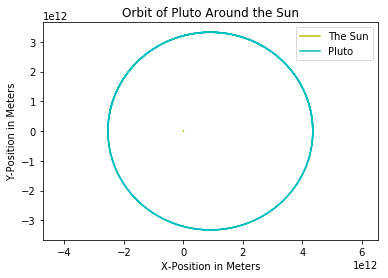
\includegraphics[width=8cm, height=5cm]{Figures/FP Pluto Orbit.png}
    \caption{\small{One Orbital Period of Pluto.}}
    \label{Fig. Pluto Orbit}
\end{figure}
\par \noindent
From Figure \ref{Fig. Pluto Orbit}, it can be seen that Pluto gets closer to the sun than when it started its orbit as it traverses through it. Once Pluto is at its closest point to the sun, it begins its journey back to perihelion. This denotes an elliptical orbit, which is exactly what Kepler's first law states. Although planetary orbits can be solved numerically, the ultimate goal is to plot three-body orbits over time. These orbits are going to be more complex than any two-body orbit. But before the three-body system is examined, a "chaotic" (A less common) scenario in which the masses do not orbit each other will be looked at next.
%---------------------------------------------------------------------------
%	Chaotic 2-Body Motion
%---------------------------------------------------------------------------
\section{Chaotic Two-Body Motion}
Consider a scenario in which a celestial body (Be it a planet, star, asteroid, etc) is at rest in space. Consider another celestial body that comes flying through space in the general vicinity of the other body of mass. In this example, the celestial body that is at rest in space has a mass of $M=2.0\cdot10^{28}$ kg were as the mass that is initially flying away from the body at rest has a mass of $m=1.0\cdot10^{22}$ kg. Comparatively, the body at rest is a star that is about a thousand times smaller than our sun and the body of mass that is flying by is a little smaller than Pluto. The smaller mass is about one astronomical unit away from the bigger mass moving away with a velocity of $v_{x}=2000$ (m/s) in the x-direction and $v_{y}=3500$ (m/s) in the y-direction. The following plot depicts the smaller body of mass' trajectory in about 4.1 years worth of time after the initial fly by.
%---------------------------------------------------------------------------
%	Figure 7 - 2 Body Fly By Fig. 1
%---------------------------------------------------------------------------
\begin{figure}[ht]
    \centering
    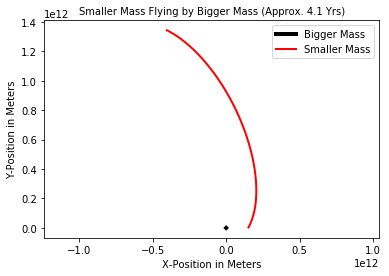
\includegraphics[width=8cm, height=5cm]{Figures/2-Body Fly By (1).png}
    \caption{\small{Smaller Mass Flying By Bigger Mass.}}
    \label{Fig. 2 Body Fly By Fig. 1}
\end{figure}
\par \noindent
Figure \ref{Fig. 2 Body Fly By Fig. 1} is meant to serve as a visual representation of what this mass' trajectory would look like shortly after starting its journey past the other massive body in space. It is shown in the early on stages in the smaller mass' trajectory that it was trying to escape the gravitational attraction of the larger mass. Over time it can also be seen that the mass is starting to return to the large mass. Over time, it should be observed that the smaller mass will orbit the larger one. Figure 8 shows one full orbit for the smaller mass around the larger mass. The time elapsed is roughly 127 years.
%---------------------------------------------------------------------------
%	Figure 8 - 2 Body Fly By Fig. 2
%---------------------------------------------------------------------------
\begin{figure}[ht]
    \centering
    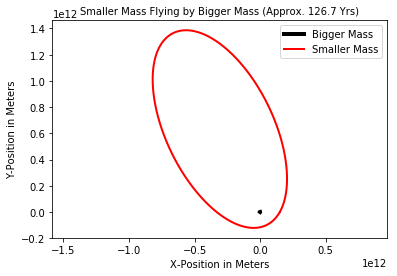
\includegraphics[width=8cm, height=5cm]{Figures/2-Body Fly By (2).png}
    \caption{\small{One Complete Orbit of Smaller Mass.}}
    \label{Fig. 2 Body Fly By Fig. 2}
\end{figure}
\par \noindent
It should be noted that this orbit is eccentric, and is far from being a circle. The purpose of Figures \ref{Fig. 2 Body Fly By Fig. 1} and \ref{Fig. 2 Body Fly By Fig. 2} is to emulate a fly by of an unbound celestial body in space. Unbound bodies can be interpreted as flying freely through space and not being bound to a body's gravitational pull such that it would orbit that body. At times when the smaller mass is closer to the bigger mass, the velocity of the smaller mass should be observed to be greater. Conversely, when the smaller mass is very far away from the larger mass it is moving at a slower rate in its orbit. Now let us consider one last scenario for two body orbital dynamics.

Instead of the larger mass staying at rest, in this scenario the larger mass is now moving away with a velocity of $v_{x}=-300$ \textit{m/s} in the x-direction and $v_{y}=75$ \textit{m/s} in the y-direction. Let the smaller mass move at the same velocities as previously stated and both masses start in their original positions as before. Both the smaller and larger mass are moving in the positive y-direction, but they are moving apart in the x-direction. We will now examine how this system evolves over time.
%---------------------------------------------------------------------------
%	Figure 9 - 2 Body Fly By Fig. 3
%---------------------------------------------------------------------------
\begin{figure}[ht]
    \centering
    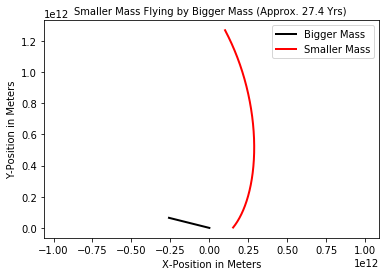
\includegraphics[width=8cm, height=5cm]{Figures/2-Body Fly By (3).png}
    \caption{\small{Bigger Mass Moving Away From Smaller Mass.}}
    \label{Fig. 2 Body Fly By Fig. 3}
\end{figure}
\par \noindent
Figure \ref{Fig. 2 Body Fly By Fig. 3} is similar to that of Figure \ref{Fig. 2 Body Fly By Fig. 1} in that the initial trajectories of both objects seem to be similar. Although they have about the same shape as one another, they are over different time intervals. The time span in Figure \ref{Fig. 2 Body Fly By Fig. 3} is about seven times longer than that of Figure \ref{Fig. 2 Body Fly By Fig. 1}'s, so it can be noted that the movement of the larger mass has a direct effect on the orbit of the smaller mass. Figure 10 shows the trajectories of both masses over an even longer time interval.
%---------------------------------------------------------------------------
%	Figure 10 - 2 Body Fly By Fig. 4
%---------------------------------------------------------------------------
\begin{figure}[ht]
    \centering
    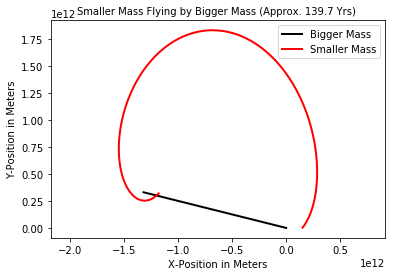
\includegraphics[width=8cm, height=5cm]{Figures/2-Body Fly By (4).png}
    \caption{\small{One Semi Orbit Around Bigger Mass.}}
    \label{Fig. 2 Body Fly By Fig. 4}
\end{figure}
\par \noindent
The time span of the orbit in Figure \ref{Fig. 2 Body Fly By Fig. 4} is approximately 13 years longer than that of Figure \ref{Fig. 2 Body Fly By Fig. 2}'s time span. Note the largest difference between the orbit in Figure \ref{Fig. 2 Body Fly By Fig. 4} and the orbit in Figure \ref{Fig. 2 Body Fly By Fig. 2} is that the smaller mass is really not orbiting the larger mass in the same way in Figure \ref{Fig. 2 Body Fly By Fig. 4} as in Figure \ref{Fig. 2 Body Fly By Fig. 2}. The smaller mass in Figure \ref{Fig. 2 Body Fly By Fig. 4} is trailing along with the larger mass as it moves throughout space. Where as the smaller mass in Figure \ref{Fig. 2 Body Fly By Fig. 2} is orbiting the larger mass in a much more predictable sense. As time progresses and this orbit is repeated, a pattern can be seen in the smaller mass' trajectory. Figure 11 shows exactly this.
%---------------------------------------------------------------------------
%	Figure 11 - 2 Body Fly By Fig. 5
%---------------------------------------------------------------------------
\begin{figure}[ht]
    \centering
    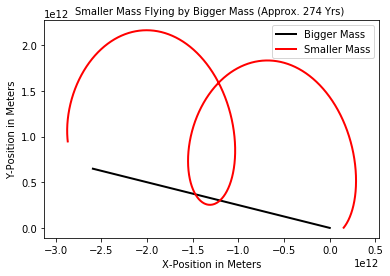
\includegraphics[width=8cm, height=5cm]{Figures/2-Body Fly By (5).png}
    \caption{\small{Two Semi Orbits of Moving Larger Mass.}}
    \label{Fig. 2 Body Fly By Fig. 5}
\end{figure}
\par \noindent
The term chaotic is really not the most appropriate way to describe the motion of these bodies. Non predictable orbits would be more of a consideration for chaotic motion. However, the motion of the bodies when both were moving just didn't look like a typical orbit. Figure \ref{Fig. 2 Body Fly By Fig. 5} shows the periodicity of the orbit as the smaller mass is about to complete two orbits in the figure. It should be noted that in two body systems most of the motion is periodic and predictable over time. As time progresses, this orbit will repeat leading it to be more stable than chaotic. In the event that a third body came into the system, the system could eventually be considered chaotic due to its unpredictable nature. This of course gives a natural extension to our main focus of study. Finally, the dynamics of three body orbits can be looked at.
%---------------------------------------------------------------------------
%	Three-Body Orbital Dynamics
%---------------------------------------------------------------------------
\section{Three-Body Orbital Dynamics}
Unlike the two-body orbital dynamics scenarios, the equations of motion for the bodies in space are more difficult to solve numerically. Instead of one body of mass only having the gravitational attraction of another single body of mass, one body of mass in a three-body orbital system will experience the force of gravity due to two other bodies of mass. This difference will cause a noticeable change of equations of motion for one body of this system. Before we examine the plots, we will first look at the math behind the three-body system orbit. We begin with clarifying notation that will be used.
\newpage
\begin{center}
$\textbf{F}_{123}$ - \small{The force on mass 1 due to masses 2 and 3}.\newline
$\textbf{F}_{213}$ - \small{The force on mass 2 due to masses 1 and 3}.\newline
$\textbf{F}_{312}$ - \small{The force on mass 3 due to masses 1 and 2}.\newline
$r_{31}$ , $r_{13}$ - \small{The distance from mass 3 to mass 1}.\newline
$r_{32}$ , $r_{23}$ - \small{The distance from mass 3 to mass 2}.\newline
$r_{21}$ , $r_{12}$ - \small{The distance from mass 2 to mass 1}.\newline
\end{center}
It should be noted that this notation will be used for the rest of the manuscript. It was previously stated that one body in this system will feel the force of two bodies on it while interacting in this system. Since this is true, the following equations result. The force equations for all three bodies of mass are;
%---------------------------------------------------------------------------
%	Equation 13 - 3 Body Eqn. Body 1
%---------------------------------------------------------------------------
\begin{equation}\label{Eqn. 3 Body Eqn. Body 1}
M_1 \Vec{\textbf{a}_1}=-\frac{GM_1M_2}{{r_{12}}^2}{\Vec{\textbf{n}}}-\frac{GM_1M_3}{{r_{13}}^2}{\Vec{\textbf{n}}},
\end{equation}
%---------------------------------------------------------------------------
%	Equation 14 - 3 Body Eqn. Body 2
%---------------------------------------------------------------------------
\begin{equation}\label{Eqn. 3 Body Eqn. Body 2}
M_2 \Vec{\textbf{a}_2}=-\frac{GM_2M_1}{{r_{21}}^2}{\Vec{\textbf{n}}}-\frac{GM_2M_3}{{r_{23}}^2}{\Vec{\textbf{n}}},
\end{equation}
%---------------------------------------------------------------------------
%	Equation 15 - 3 Body Eqn. Body 3
%---------------------------------------------------------------------------
\begin{equation}\label{Eqn. 3 Body Eqn. Body 3}
M_3 \Vec{\textbf{a}_3}=-\frac{GM_3M_1}{{r_{31}}^2}{\Vec{\textbf{n}}}-\frac{GM_3M_2}{{r_{32}}^2}{\Vec{\textbf{n}}}.  
\end{equation}
Once the value for the unit vector in equations (\ref{Eqn. 3 Body Eqn. Body 1})-(\ref{Eqn. 3 Body Eqn. Body 3}) is substituted in, the equations of motion become difficult to solve analytically. It should be noted that it is assumed that these bodies of mass are not changing in mass thus the only kind of change in momentum that can occur in this system is an acceleration of one of the bodies of mass.
%---------------------------------------------------------------------------
%	Figure 12 - 3-Body Cartoon Fig. 1
%---------------------------------------------------------------------------
Figure 12 illustrates the initial position of our three-body system.
\begin{figure}[ht]
    \centering
    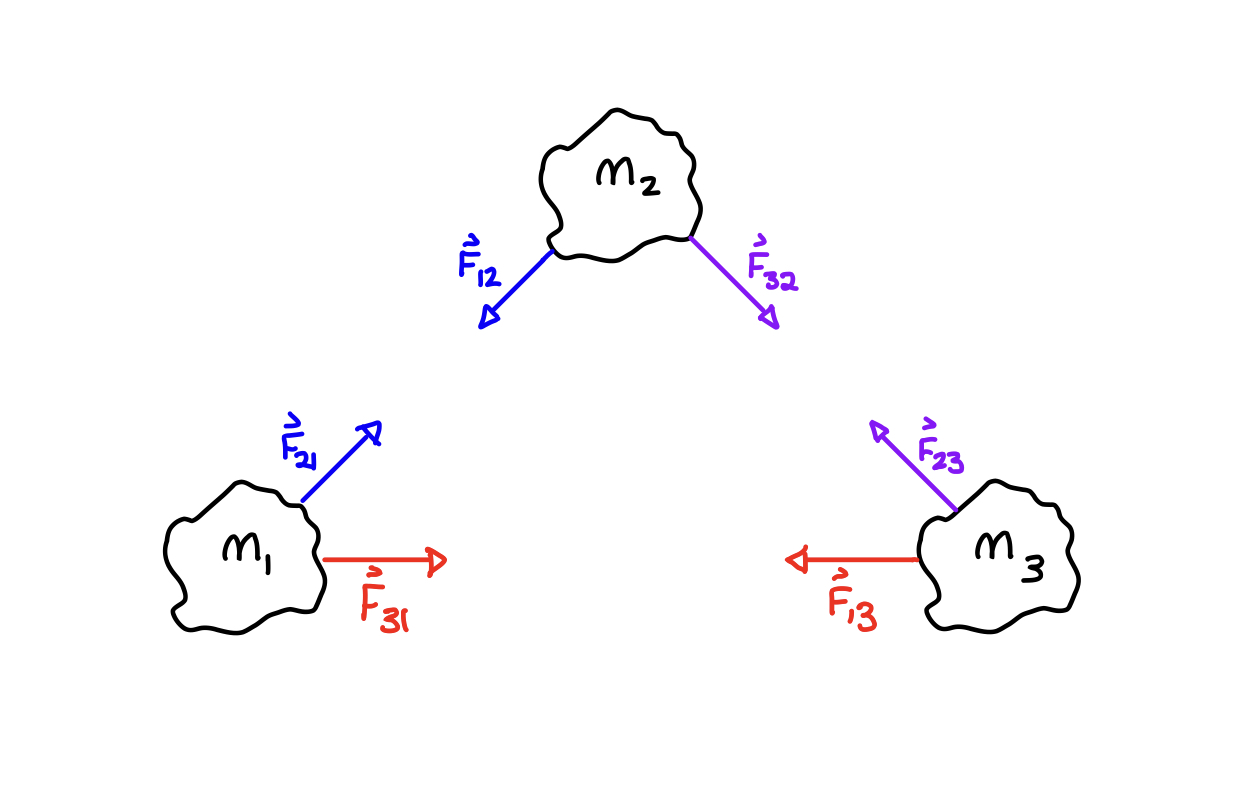
\includegraphics[width=8cm, height=5cm]{Figures/3-Body Cartoon (1).png}
    \caption{\small{A Configuration of Three Massive Bodies in Space Interacting.}}
    \label{Fig. 3-Body Cartoon Fig. 1}
\end{figure}
\par \noindent
Examining configurations similar to Figure \ref{Fig. 3-Body Cartoon Fig. 1}, the trajectories of the masses can be plotted with the use of Python and numerical integration techniques. We first examine what happens to three bodies of mass when the largest mass is moving away from the two smaller masses.
\newpage
%---------------------------------------------------------------------------
%	Figure 13 - 3-Body Dynamics Fig. 1
%---------------------------------------------------------------------------
\begin{figure}[ht]
    \centering
    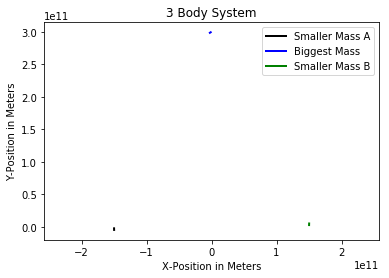
\includegraphics[width=8cm, height=5cm]{Figures/3-Body Dynamics (1).png}
    \caption{\small{Initial Location of Three Masses.}}
    \label{Fig. 3-Body Dynamics Fig. 1}
\end{figure}
\par \noindent
Figure \ref{Fig. 3-Body Dynamics Fig. 1} shows the starting points of these bodies of mass. The configuration of these three bodies of mass was so that they would form an equilateral triangle. The separation distance between the three bodies of mass is equidistant. The two smaller masses (The black and green dots) are positioned one astronomical unit apart on the x-axis from the origin in each direction (One at $x=-1.0$ AU and $x=1.0$ AU). The units that appear in Figure \ref{Fig. 3-Body Dynamics Fig. 1} are in meters rather than astronomical units. The biggest mass is positioned so that it bisects the two smaller masses on the x-axis but is one astronomical unit from the origin in the y-direction. Now lets consider when the two smaller masses are at rest with the larger mass also at rest.
%---------------------------------------------------------------------------
%	Figure 14 - 3-Body Dynamics Fig. 2
%---------------------------------------------------------------------------
\begin{figure}[ht]
    \centering
    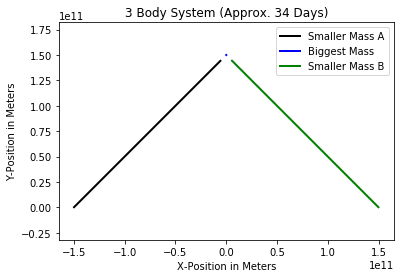
\includegraphics[width=8cm, height=5cm]{Figures/3-Body Dynamics (2).png}
    \caption{\small{The Accretion of Smaller Masses by a Larger Mass.}}
    \label{Fig. 3-Body Dynamics Fig. 2}
\end{figure}
\par \noindent
The masses in Figure \ref{Fig. 3-Body Dynamics Fig. 2} were configured so that the smaller ones (The green and the black) were approximately the same mass as Earth ($m_E\approx6.0\cdot10^{24}$ Kg). The largest mass was made so that it would be approximately the same mass as the Sun ($m_s\approx2.0\cdot10^{30}$ Kg). It should come with no surprise that both of these masses are attracted towards the larger mass, so strongly that they traverse in a straight line to the larger mass. Figure \ref{Fig. 3-Body Dynamics Fig. 2} confirms what we should expect to see happen. We next examine the evolution of the system when the masses are initially at rest.

Let's look at the same configuration of the masses that can be seen in Figure \ref{Fig. 3-Body Dynamics Fig. 1}. Instead of the smaller mass ($M_1$) positioned at ($-1.0$ AU, 0) being at rest, it is moving initially at $V_{0x}=30,000$ $\frac{m}{s}$ in the positive x-direction. As for the other smaller mass ($M_3$) positioned at ($1.0$ AU, 0), it is moving initially at $V_{0y}=30,000$ $\frac{m}{s}$ in the positive y-direction. With the larger mass ($M_2$) positioned at the same spot as before and stationary, Figure 15 simulates the trajectories of the planets.
%---------------------------------------------------------------------------
%	Figure 15 - 3-Body Dynamics Fig. 3
%---------------------------------------------------------------------------
\begin{figure}[ht]
    \centering
    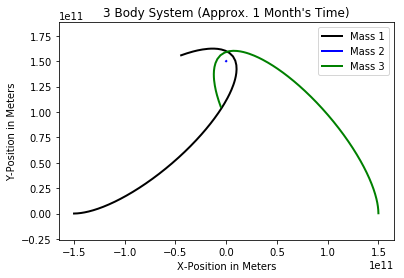
\includegraphics[width=8cm, height=5cm]{Figures/3-Body Dynamics (3).png}
    \caption{\small{Trajectories Over A Month.}}
    \label{Fig. 3-Body Dynamics Fig. 3}
\end{figure}
\par \noindent
Figure \ref{Fig. 3-Body Dynamics Fig. 3} shows that the two masses follow similar paths. Considering both of these masses orbiting Mass 2 are the same mass, we should expect to see similar trajectories over time. Figure 16 shows the orbit of these two bodies over a greater length of time.
%---------------------------------------------------------------------------
%	Figure 16 - 3-Body Dynamics Fig. 4
%---------------------------------------------------------------------------
\begin{figure}[ht]
    \centering
    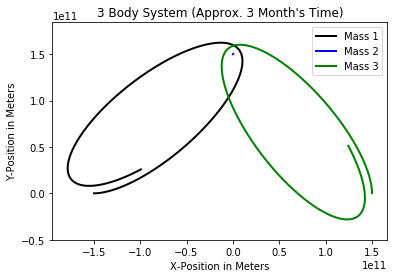
\includegraphics[width=8cm, height=5cm]{Figures/3-Body Dynamics (4).png}
    \caption{\small{Trajectories Over Three Months.}}
    \label{Fig. 3-Body Dynamics Fig. 4}
\end{figure}
\par \noindent
The orbits of masses 1 and 3 follow the same general shape throughout. The orbits of these two planets are elliptic due to the initial conditions of the planets. As time progresses, the orbit seems to change in shape slightly where the planet is not traversing the same exact path through each orbit.  This precision of the planets can be seen very easily over a longer time span. Looking at the same scenario as in Figure \ref{Fig. 3-Body Dynamics Fig. 2} and \ref{Fig. 3-Body Dynamics Fig. 3}, Figure \ref{Fig. 3-Body Dynamics Fig. 4} is generated over a three year time span.
\newpage
%---------------------------------------------------------------------------
%	Figure 17 - 3-Body Dynamics Fig. 5
%---------------------------------------------------------------------------
\begin{figure}[ht]
    \centering
    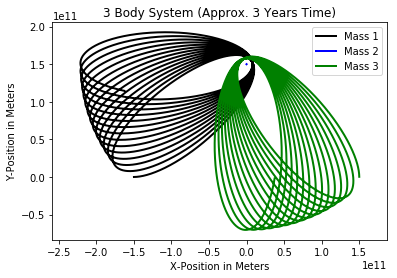
\includegraphics[width=8cm, height=5cm]{Figures/3-Body Dynamics (5).png}
    \caption{Precision of Planets Over Three Years.}
    \label{Fig. 3-Body Dynamics Fig. 5}
\end{figure}
\par \noindent
We should expect to see this same pattern throughout time assuming that no other large mass comes into the system to interfere. If the planets were to come close to one another, their orbits would change and this system would become chaotic. Thankfully due to the initial conditions in this example the orbits will not be interfered with.

Considering the previous scenario as in Figure \ref{Fig. 3-Body Dynamics Fig. 1} we will now look at a dynamic system of these bodies of mass. The first thing that will be different from the previous scenarios are the masses of the celestial bodies in this system. The two smaller masses in the system ($M_1$ and $M_3$) are now both $6.0\cdot10^{26}$ Kg where as the biggest mass ($M_2$) is now $2.0\cdot10^{31}$ Kg. $M_1$ and $M_3$ are both set in motion at $V_{0y}=30,000$ $\frac{m}{s}$ where as $M_2$ is set in motion at $V_{0y}=-30,000$ $\frac{m}{s}$. With these differences from before, the following plot is generated of the three bodies and their trajectories.
%---------------------------------------------------------------------------
%	Figure 18 - 3-Body Dynamics Fig. 6
%---------------------------------------------------------------------------
\begin{figure}[ht]
    \centering
    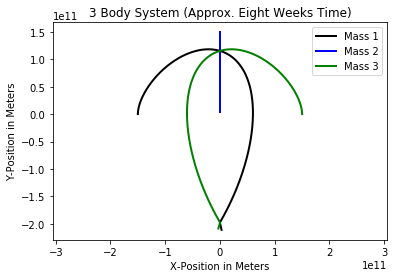
\includegraphics[width=8cm, height=5cm]{Figures/3-Body Dynamics (6).png}
    \caption{\small{Three Bodies in Motion.}}
    \label{Fig. 3-Body Dynamics Fig. 6}
\end{figure}
\par \noindent
As these bodies move through space, $M_2$ originally attracts both $M_1$ and $M_3$ due to its gravitational attraction. After this initial attraction, the smaller masses are 'sling-shotted' past the larger mass and continue onward in their trajectories. The main reason for this trajectory is due to the motion of the larger mass. Because of this, the trajectories are different from those seen in Figures \ref{Fig. 3-Body Dynamics Fig. 3}-\ref{Fig. 3-Body Dynamics Fig. 5}. With this large body of mass, we now start to see more chaotic orbits from the smaller masses. After approximately five months in time, Figure 19 is generated for the three bodies and their trajectories.
%---------------------------------------------------------------------------
%	Figure 19 - 3-Body Dynamics Fig. 7
%---------------------------------------------------------------------------
\begin{figure}[ht]
    \centering
    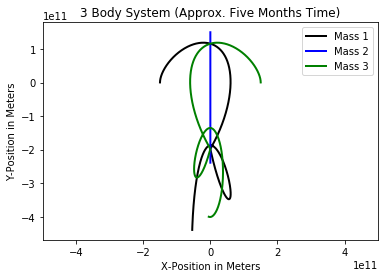
\includegraphics[width=8cm, height=5cm]{Figures/3-Body Dynamics (7).png}
    \caption{\small{Three Bodies in Motion.}}
    \label{Fig. 3-Body Dynamics Fig. 7}
\end{figure}
\par \noindent
After $t=5$ months, the orbits become chaotic. The larger mass can be seen to having a prominent effect on the smaller masses but at certain points in the orbit the two smaller masses influence each other. Examining this same system we should expect to see chaotic behavior continuing as time goes on. After one year, Figure 20 shows the plot of the bodies and their trajectories.
%---------------------------------------------------------------------------
%	Figure 20 - 3-Body Dynamics Fig. 8
%---------------------------------------------------------------------------
\begin{figure}[ht]
    \centering
    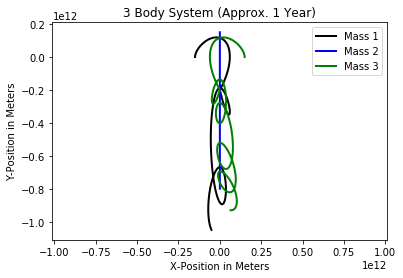
\includegraphics[width=8cm, height=5cm]{Figures/3-Body Dynamics (8).png}
    \caption{\small{Three Bodies in Motion Over One Year.}}
    \label{Fig. 3-Body Dynamics Fig. 8}
\end{figure}\
\par \noindent
Figure \ref{Fig. 3-Body Dynamics Fig. 8} shows an absence of a pattern, thus leading the orbit to be considered chaotic. The only mass that stays constant is the huge mass that is only moving in the negative y-direction. All of the plots found in Figures \ref{Fig. 3-Body Dynamics Fig. 1}-\ref{Fig. 3-Body Dynamics Fig. 8} involve masses that have one with a substantially higher mass than the other two. In systems where there are three bodies in motion, it is evident that these orbits are not stable. This is not true for all three body systems, but it is true for the majority of the systems. 

Now that the equidistant scenario has been covered, a different initial configuration of these three bodies in space will now be examined. Much like Figure \ref{Fig. 2-Body Cartoon} and Figure \ref{Fig. 3-Body Cartoon Fig. 1}, Figure 21 illustrates the force attraction of this new configuration of masses.
%---------------------------------------------------------------------------
%	Figure 21 - 3-Body Cartoon Fig. 2
%---------------------------------------------------------------------------
\begin{figure}[ht]
    \centering
    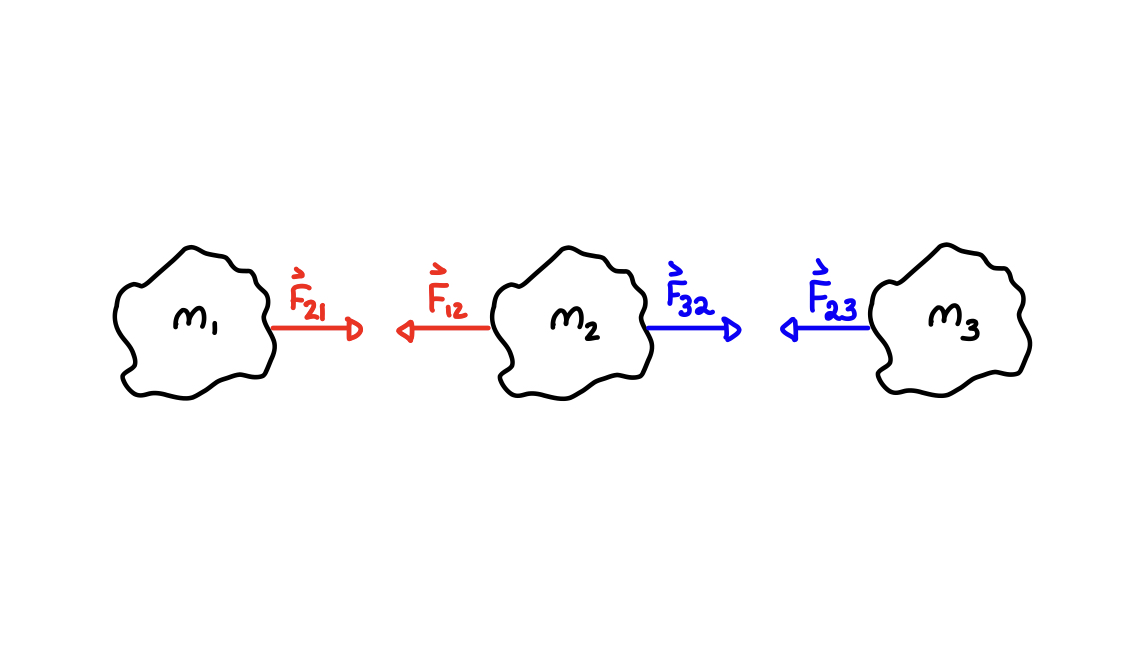
\includegraphics[width=8cm, height=4.75cm]{Figures/3-Body Cartoon (2).png}
    \caption{\small{Initial Configuration of Three Bodies in Space.}}
    \label{Fig. 3-Body Cartoon Fig. 2}
\end{figure}
\begin{center}
\end{center}
\newpage \noindent
$M_1$ and $M_3$ are now $6.0\cdot10^{29}$ Kg where $M_2$ is $2.0\cdot10^{31}$ Kg. Figure 22 depicts the initial positions of these bodies in space as a plot. All of the masses are positioned such that they are one astronomical unit away from one another. 
%---------------------------------------------------------------------------
%	Figure 22 - 3-Body Dynamics Fig. 9
%---------------------------------------------------------------------------
\begin{figure}[ht]
    \centering
    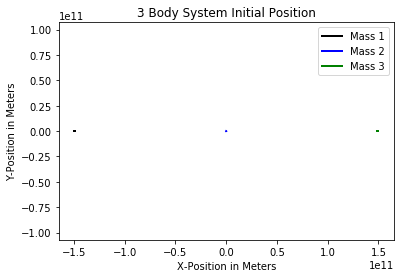
\includegraphics[width=8cm, height=4.75cm]{Figures/3-Body Dynamics (9).png}
    \caption{\small{Three Bodies Initially At Rest.}}
    \label{Fig. 3-Body Dynamics Fig. 9}
\end{figure}
\par \noindent
$M_1$ in Figure \ref{Fig. 3-Body Dynamics Fig. 9} is set in motion with a velocity of $V_{0y}=50,000$ $\frac{m}{s}$ and $M_3$ is moving at $V_{0y}=-50,000$ $\frac{m}{s}$. $M_2$ is initially at rest and is only influenced due to the other masses. 
%---------------------------------------------------------------------------
%	Figure 23 - 3-Body Dynamics Fig. 10
%---------------------------------------------------------------------------
\begin{figure}[ht]
    \centering
    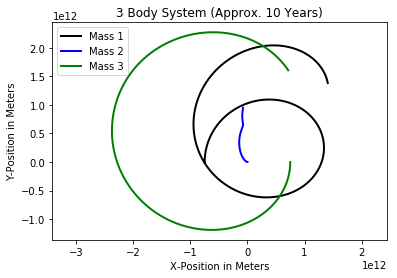
\includegraphics[width=8cm, height=4.75cm]{Figures/3-Body Dynamics (10).png}
    \caption{\small{Three Bodies in Motion After 10 Years.}}
    \label{Fig. 3-Body Dynamics Fig. 10}
\end{figure}
\par \indent
Figure \ref{Fig. 3-Body Dynamics Fig. 10} shows that the trajectories of the two masses are different looking even though they are both of the same mass in this 10 year time span. The motion that is seen of $M_2$ is due to the gravitational attraction from $M_1$ and $M_3$. The largest mass proceeds in a nonuniform trajectory much like the smaller masses do when they are orbiting the larger mass. $M_1$ makes one revolution around $M_2$ where as $M_3$ is taking a longer time to do so. This could partly be due to the initial direction of both masses and the proceeding direction of $M_2$. It is because of this non uniformity that makes this system chaotic. The orbits are not predictable like the planets in our solar system, they are sporadic with no distinguishable pattern behind them. As we let this system evolve, we see sporadic behavior that can't be predicted. Figure 24 shows the plot of the scenario in Figure \ref{Fig. 3-Body Dynamics Fig. 9} twenty years after the initial start of the orbits.
%---------------------------------------------------------------------------
%	Figure 24 - 3-Body Dynamics Fig. 11
%---------------------------------------------------------------------------
\begin{figure}[ht]
    \centering
    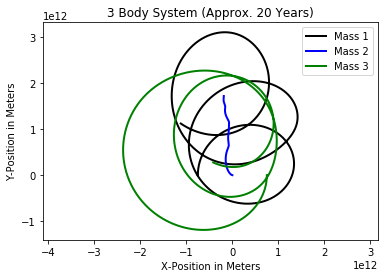
\includegraphics[width=8cm, height=4.75cm]{Figures/3-Body Dynamics (11).png}
    \caption{\small{Three Bodies in Motion After 20 Years.}}
    \label{Fig. 3 Body Dynamics}
\end{figure}
\par \noindent
Figure \ref{Fig. 3 Body Dynamics} shows the chaotic motion that is observed in three body systems. The changing of position, velocity, and acceleration in these systems are what cause the chaotic behavior that we observe in the plots. When there is a greater difference in mass in the system, as in Figures \ref{Fig. 3-Body Dynamics Fig. 1}-\ref{Fig. 3-Body Dynamics Fig. 8}, the orbits of the other bodies tend to be more planetary and can be predicted with a lot more accuracy. This only changes when the largest mass is set in motion as well. 

There is one last scenario to examine for the three body system. First the masses of of the bodies will be changed. $M_1$ and $M_2$ are both now $2.0\cdot10^{29}$ Kg and $M_3$ is now $2.0\cdot10^{31}$ Kg. The purpose of these mass configurations are to attempt to create a stable orbit in the system. The mass of the largest body is only 100 times greater than that of the smaller masses, compared to the mass ratio of about 3.3 million as seen in Figures \ref{Fig. 3-Body Dynamics Fig. 1}-\ref{Fig. 3-Body Dynamics Fig. 8}. Taking the same initial positions of the bodies in space as in Figure \ref{Fig. 3-Body Dynamics Fig. 9}, $M_1$ is set in motion at $50,000$ $\frac{m}{s}$ in the y-direction and the $M_3$ at $50,000$ $\frac{m}{s}$ in the negative y-direction. Taking these new parameters into account, Figure 25 is generated for these bodies' trajectories.
\newpage
%---------------------------------------------------------------------------
%	Figure 25 - 3-Body Dynamics Fig. 12
%---------------------------------------------------------------------------
\begin{figure}[ht]
    \centering
    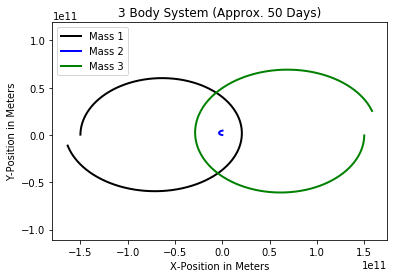
\includegraphics[width=8cm, height=4.75cm]{Figures/3-Body Dynamics (12).png}
    \caption{\small{Three Bodies in Motion After 50 Days.}}
    \label{Fig. 3-Body Dynamics Fig. 12}
\end{figure}
\par \noindent
Figure \ref{Fig. 3-Body Dynamics Fig. 12} shows that the both $M_1$ and $M_3$ traverse similar paths over this 50 day interval. As time progresses in this orbit, the largest mass is only influenced by the two smaller masses. Because of this fact, $M_2$ follows the same path throughout time. Only $M_1$ and $M_3$ have trajectories that are different over time. Figure 26 shows this progression over one year.
%---------------------------------------------------------------------------
%	Figure 26 - 3-Body Dynamics Fig. 13
%---------------------------------------------------------------------------
\begin{figure}[ht]
    \centering
    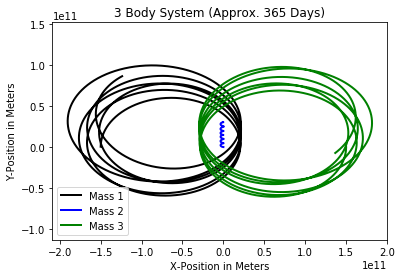
\includegraphics[width=8cm, height=4.75cm]{Figures/3-Body Dynamics (13).png}
    \caption{\small{Three Bodies in Motion After One Year.}}
    \label{Fig. 3-Body Dynamics Fig. 13}
\end{figure}
\par \noindent
After one years time, the orbits of $M_1$ and $M_3$ start to deviate in the path that they traverse. When the two smaller bodies of mass are in close vicinity of one another, the path gets altered due to the gravitational attraction of each mass. It is because of this that the orbit is considered to be chaotic. Figure 27 shows this orbit over two years.
%---------------------------------------------------------------------------
%	Figure 27 - 3-Body Dynamics Fig. 14
%---------------------------------------------------------------------------
\begin{figure}[ht]
    \centering
    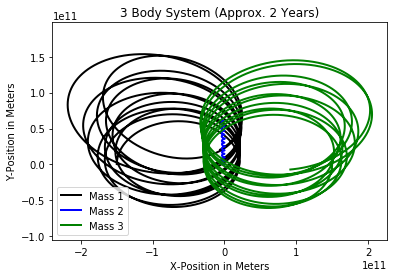
\includegraphics[width=8cm, height=4.5cm]{Figures/3-Body Dynamics (14).png}
    \caption{\small{Three Bodies in Motion After Two Years.}}
    \label{Fig. 3-Body Dynamics Fig. 14}
\end{figure}
\newpage \noindent
Figure \ref{Fig. 3-Body Dynamics Fig. 14} shows that these orbits are progressively becoming chaotic with the orbits changing over time. Finally, Figure 28 illustrates the chaotic nature of this system after four years.
%---------------------------------------------------------------------------
%	Figure 28 - 3-Body Dynamics Fig. 15
%---------------------------------------------------------------------------
\begin{figure}[ht]
    \centering
    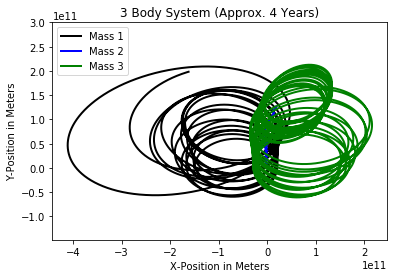
\includegraphics[width=8cm, height=5cm]{Figures/3-Body Dynamics (15).png}
    \caption{\small{Three Bodies in Motion After Four Years.}}
    \label{Fig. 3-Body Dynamics Fig. 15}
\end{figure}
\par \noindent
Figures \ref{Fig. 3-Body Dynamics Fig. 13}-\ref{Fig. 3-Body Dynamics Fig. 15} help illustrate that these orbits are not stable, and that in fact they are chaotic.
%---------------------------------------------------------------------------
%	Conclusion
%---------------------------------------------------------------------------
\section{Conclusion}
We solved for the motion of the three body system numerically with the use of a Forward Euler Difference Scheme. This was first accomplished by solving for the time that it would take for a ball to hit the ground due to gravitational acceleration of the Earth. After this scenario, the two-body system was solved. These systems covered semi traditional orbits (Like the Earth and Pluto around the Sun) and also more nontraditional orbits like a planet following star moving in a linear direction. Once the two-body problem was solved, the three-body system was then solved. It was in these systems that we found our most chaotic behavior among the bodies in the system. In these systems of three-body orbits, stable orbits are near impossible to simulate. It is because of this that most of these systems are chaotic and tend to not be stable over time. With infinite different initial conditions for these systems, there are also infinite solutions for these systems.
%---------------------------------------------------------------------------
%	Bibiliography
%---------------------------------------------------------------------------
\clearpage
\twocolumn[
    \begin{@twocolumnfalse}
       \begin{thebibliography}{2}
           \bibitem{Marion}
            Marion, Thornton. Classical Dynamics. Boston: Cengage Learning, 2018.
            \bibitem{BodyWiki}
            Wikipedia. Wikipedia. 15 October 2018. November 2018. \url{https://en.wikipedia.org/wiki/Three-body_problem}.
       \end{thebibliography} 
    \end{@twocolumnfalse}
]
\end{document}